\chapter{Test scenario and evaluation}
\label{chap:testscenarioandevaluation}

Both, the visual language and the automated constraint generation functionality, have been integrated into Robostudio in order to evaluate the proposed safety functionality. Robostudio is a visual programming environment which allows the specification of state machine based programs whose behaviour can then be examined by visual constraints.
As a test scenario the simplified medication reminder application is considered whose underlying screen-flow is explained in figure~\ref{fig:medicationreminder}. Starting from ``Menu'' the user can choose from several services such as blood pressure measurement or entertainment. In the given example these services are simplified to just one state ``additional services'' since the focus concentrates on the medication reminder part. In state ``Polling'' the database is checked for a pending reminder and, if there is one, the medication intake guidance is triggered. The patient can state if he or she has already taken the medication, or decide whether to take it or not. In the latter case, he or she may give a reason for it and a caregiver is notified about this incident. Otherwise the progress will result in the state ``Well done!'' after completing intake.

\begin{figure}[htbp]
  \centering
  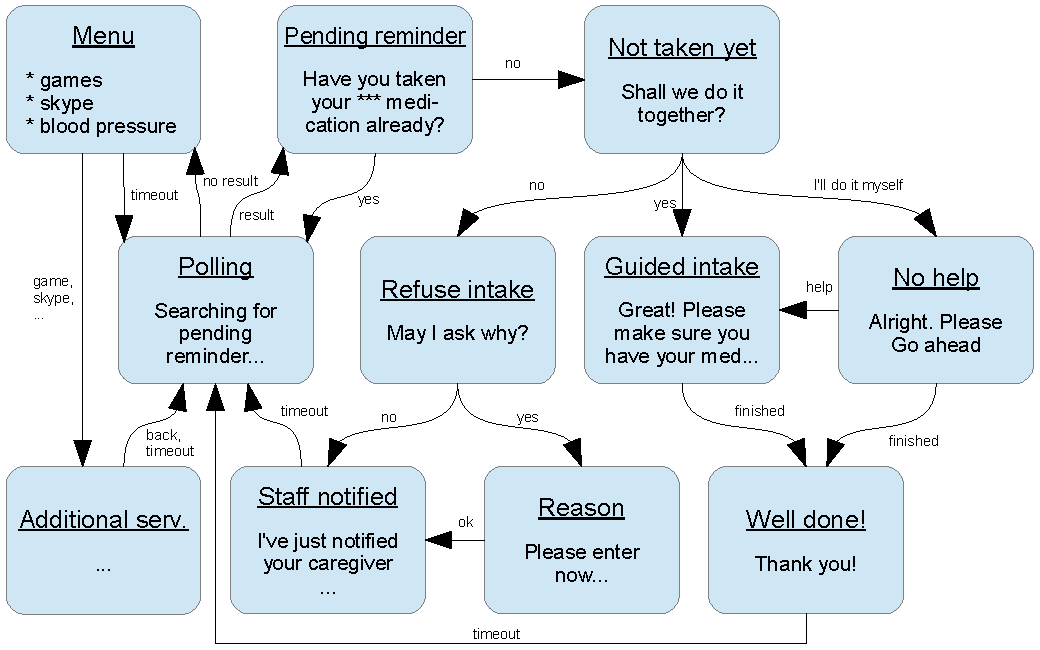
\includegraphics[width=\linewidth]{stm.pdf}
  \caption{Simplified screen-flow of the medication reminder application.}
  \label{fig:medicationreminder}
\end{figure}

This state machine with all its states, transitions and screen dialogs has been implemented in Robostudio and in the following sections we will evaluate the visual language as well as the potential of constraint generation. Section~\ref{sec:practicalexperiences} describes how a non-expert deals with the visual language and what the final judgement is.



\section{Operator constraints}

Before constraints can be created it might be useful to think about a reasonable term to express. Let's take the example ``Whenever there is a pending reminder, medication will be finally taken or caregivers will get notified in case of the patient refusing medication intake.'' given as a requirement in chapter~\ref{chap:goals}.

In order to find a corresponding graphical constraint the sentence has to be analyzed just as developers read it. Since ``whenever'' is a semantic equivalent to ``always if'' first of all a \emph{ALWAYS} operator gets dragged to the dashboard directly followed by an \emph{IF} as shown in figure~\ref{fig:sampleconstraint}. The condition for this \emph{IF} is that there is a pending reminder, so a state ``Not taken yet'' has to be added to the upper bucket of the \emph{IF} operator.
Whenever the just mentioned condition becomes true, there also has to be true in future: Medication is taken properly or caregivers get notified about refuse. Accordingly a \emph{FUTURE} operator containing an \emph{OR} forms the second part of the \emph{IF} operator. Finally two states 'Well done!' and 'Staff notified' get added to the disjunction. The resulting visual constraint can now automatically be translated to the corresponding LTL formula by the editor:

\begin{equation} \label{eq:sampleconstraint}
  \models \Box (\textnormal{'Not taken yet'} \Rightarrow \Diamond (\textnormal{'Well done!'} \vee \textnormal{'Staff notified'}))
\end{equation}

\begin{figure}[htbp]
  \centering
  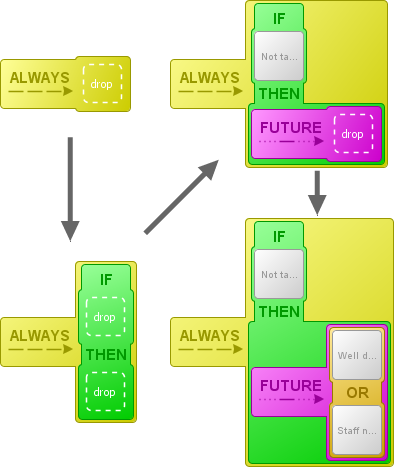
\includegraphics[scale=0.65]{sampleconstraint}
  \caption{Visual constraint creation for LTL formula ~\ref{eq:sampleconstraint}.}
  \label{fig:sampleconstraint}
\end{figure}

After each change in the dashboard, the constraint is automatically recompiled and revalidated by using the underlying model checker. For syntactically invalid constraints, an ``incomplete'' sign is displayed in the respective tab. Otherwise, an animated ring indicates that validation is in pro\-gress and will finally result in either a ``valid'' or ``invalid'' sign.



\subsection{Usability}

Due to the optimized performance of NuSMV, even the validation of constraints on huge and complex programs is fast and allows rapid feedback. In addition, the validation itself runs in the background without locking the dashboard. Therefore waiting times and disruptions during constraint development can be avoided, which would be likely with conventional model checking where constraint development and constraint validation are alternating processes. Thus our tool is considered an improvement for the user experience.

It could be observed that the different color flavours of the visual operators are a good support for fast reading and understanding of constraints. Also the two dimensional composition and the round shapes of the operators turned out to give the language a schematic but not too rectangular look. Besides it is considered eye-candy what is the best motivation for using this visual language.





\subsection{Expressiveness}

Due to being based on LTL, the visual language's expressivenes is equivalent to LTL's one of course. More precisely this means any temporal logic formula can be expresssed except potentiality.
Furthermore there is one more limitation in the current visual language concerning the variety of available proposition operators. The visual language was originally designed for validating healthcare applications where just one kind of proposition is needed: ``currently state x is active''. Thus other propositions such as equations, greater than etc. are not implemented yet, but can be easily integrated.
Figure~\ref{fig:example_propositions} depicts how an extension of \emph{LTLCreator} with additional proposition operators could be realised.

\begin{figure}[htbp]
  \centering
  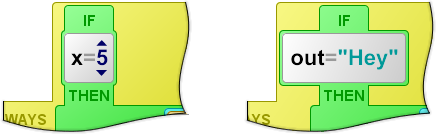
\includegraphics[scale=0.65]{example_propositions}
  \caption{Possible proposition extensions: numeric and string equations.}
  \label{fig:example_propositions}
\end{figure}



\section{Automated constraint generation}

The automated constraint generation can be triggered by a click on the magic wand button in the tab area. After activation a dashboard is opened in a new tab for each constraint found, and validation is initiated immediately. For the medication reminder application six constraints are found, including \emph{a)} and \emph{b)} shown in figure~\ref{fig:generatedconstraints} which match the postulations in the requirements in chapter~\ref{chap:goals}.
The constraint used for demonstration in the previous section is also generated, however \emph{b)} forms an intensified restriction of it. 
Constraint \emph{a)} ensures the ``Polling'' state is always eventually visited again. If a pending medication is not already taken, constraint \emph{b)} guarantees intake or staff notification before the next reminders can be read from the database.

The search and generation process finishes within less than a second and thus doesn't let developers wait for a long time.

It was showed that the subgraph approach is working for the medication reminder application, and there was even one more reasonable constraint found by the heuristic: Constraint \emph{c)} ensures that during the medication intake process the program can not switch back to the menu or other services such as entertainment or blood pressure measurement.



\begin{figure}[htbp]
  \centering
  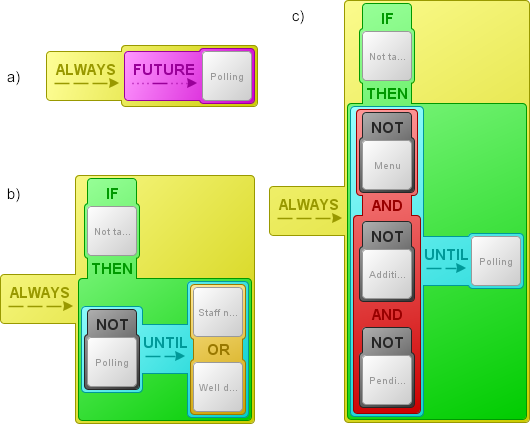
\includegraphics[scale=0.65]{generatedconstraints}
  \caption{Automatically generated constraints which match the required postulations.}
  \label{fig:generatedconstraints}
\end{figure}






\subsection{Performance}

In order to examine the performance of subgraph finding and constraint generation, we need to have a second look at the implementation details again. The subgraph finding algorithm is realized similar to a depth-first search. Indeed all healthcare programs are infinite and contain cycles and a depth-first walk-through would never end, but as stated in section~\ref{sec:prototype:automatedconstraintgeneration} the algorithm does not revisit already visited states.

The performance of this algorithm of course highly depends on the grade of branching. In contrast to a usual depth-first search in trees, the modified depth-first search is applicable for even cyclic state machines and will walk through all possible paths starting from one particular start state without visiting states twice. Assuming the worst case in which every state has transitions to all other states, each of the remaining $|V|-1$ states can be possibly visited next, similarly $|V|-2$ for the third step and so on. As a worst case execution time the following result is obtained:

%Nevertheless, such a depth-first search has a worst case execution time of $O(|V|+|E|)$ in which $|V|$ is the number of states and $|E|$ number of edges respective transitions in our case.
%Since we cope with state machines and thus have directed edges rather than undirected ones, each state can have $|V|$ transitions; $|V|-1$ to other ones and one to itself. For the contained tree without cycles for depth-first search we retreive $|E|=|V|$ edges.
%As worst case ececution time for the depth-first search we obtain the following result:

\begin{equation}
O(\textnormal{``depth-first search''})=O(1*(|V|-1)*(|V|-2)*...*2*1)=O((|V|-1)!)
\end{equation}

In order to find a subgraph with the presented algorithm the depth-first search has to be startet on a start state of a subgraph. Since we don't know in beforehand which states might be possible candidates for such start states, the algorithm has to be applied on every single state of the program which has two ore more outgoing transitions. In the worst case all $|V|$ states fulfil this condition, so the depth-first search has to be executed $|V|$ times. This implies for the estimated worst case execution time:

\begin{equation}
O(\textnormal{``subgraph finding''})=O(|V|)*O((|V|-1)!)=O(|V|!)
\end{equation}



\subsection{Scalability}

For all the healthcare applications that we examined the presented algorithm works efficient and fast. But their program sizes are still quite manageable. The test program has eleven states, an average branch grade of $1.\overline{63}$ outgoing transitions per state and a constraint finding execution time of a split second on a standard computer.
Of course an exponential or factorial execution time is bad if the number of states arises. A clear slowdown can be felt when the algorithm runs on larger state machines with plenty of states and a high grade of branching. A test on a state machine with over 250 states and partially high branch grade resulted in approximately five minutes execution time.

However, in case that this algorithm is used for other huge programs regardless its tailoring to the healthcare domain, it keeps a lot of potential to be improved in efficiency. With a sophisticated approach it might be enough to execute just one depth-first search for finding all subgraphs at once what would lead to a linear execution time.
% wenn noch schreiben will, dann: linear ist cool, weil das tool eh die gefundenen constraints gleich anzeigt und nicht erst am ende alles geballt bringt.



\subsection{Reasonability of generated constraints}

The constraint generator algorithm found six constraints for the medication reminder application. Two of them were actually the ones proposed in the requirements. Three of them are either intensified versions of the previous ones or just describe the behaviour of the program and thus make sense, but in matters of safety they aren't fundamental relevant.
Nevertheless the generator tool actually found a new important constraint which had not been considered before. It is constraint \emph{c)} in figure~\ref{fig:generatedconstraints}, section~\ref{sec:prototype:automatedconstraintgeneration}.

To put it in a nutshell, in context of this example all automatically generated constraints are practical, and approximately half of them are significant. This shows that the constraint generator concept works well for the healthcare application and can be a very helpful feature.




\section{Practical experiences}
\label{sec:practicalexperiences}

Some parts of the healthcare robot's behaviour are appropriate to be specified by non-programmers, and that's the purpose of the presented visual language as well. Different tools and environments, among Robostudio and LTLCreator, try to provide a particular interface suitable for such people. Now, it might be interesting to find out about user's experiences and how they get along when using these tools.

The LTLCreator has been presented to several people, technical engineers as well as ordinary persons. The overall feedback was good and the idea and realisation of the visual language was well-received. One of the laypersons who have been introduced to LTLCreator was Alina Kracker. The 21 yeras old german student of educational science is also working for the elderly in a care facility since more than five years. In this social institution Ms Kracker takes care of persons having different disease patterns and necessities. This spectrum varies from physical disabilities over mental problems such as Alzheimer's desease to being bedridden.
Her professional care background makes her feedback about usability and comprehensibility of the visual concept especially interesting since its application and testing was done in the healthcare domain.

Ms Kracker was introduced to the example of medication remider, and the program behaviour was described with the help of figure~\ref{fig:medicationreminder}. Afterwards she got familiarized with surface and functionality of LTLCreator. Now, she was asked to formulate the two constraints which we postulated in the requirements, just by using the available means of the editor placed at her disposal.
The first constraint, which ensures the state ``Polling'' always eventually to be visited again, was constructed quickly and accurately.
The second constraint specifies, that every visit of state ``Not taken yet'' will eventually result in a visit of either state ``Well done!'' or ``Staff notified''. It turned out that this constraint held some difficulties for her, the \emph{FUTURE} operator was not considered initially. But it was also finisehd after a few consideration breaks.

Ms Kracker didn't know in beforehand what state machines are and never came in contact with LTL or model checking in general. But she dealt with this example and the visual language surprisingly well, and she's convinced that she could use it after some exercise. As reason for the success she pointed out the easy readability of the visual language and its close relationship to spoken language. Furthermore the intuitive drag and drop allowed faster editing.
Her examination on the visual language gives us evidence that we succeeded with our approach of creating an easy to use concept for defining LTL formulas. The visual language we developed enables even non-professionals to use the usually quite complex concept of model checking.

To the question, whether she would recommend such robotic services like the medication reminder application for use in the care facility she's working in, Ms Kracker replied: ``I can envision such robot applications beeing an excellent assistance for the elderly who are mentally fit but maybe a little doolally. However, in our facilities most of the patients aren't capable enough anymore of making decisions based on what the robots ask. In fact, due to frequent changes of the patients in our facilities it is a big issue for the care givers not to forget time-dependend medication intakes of their patients. Thus such a reminding robot application would constitute an excellent support for us staff!''.